% Estado del arte
\chapter{Estado del arte}
\section{Tecnologías de virtualización}
Se podría decir que la virtualización es ya uno de los pilares fundamentales del mundo IT debido a las grandes ventajas que proporciona. Previo al desarrollo de las tecnologías y tipos de virtualización disponibles, es conveniente explicar en qué consiste la virtualización, que no es más que una representación mediante software de un entorno físico o recurso tecnológico, como pueden ser aplicaciones, servidores o almacenamiento.~\cite{virt1} 

Gracias a esta tecnología, es posible contar con varios ordenadores virtuales en el mismo hardware, donde cada uno de ellos puede interactuar de forma independiente y ejecutar sistemas operativos o aplicaciones diferentes mientras comparten los recursos de una sola máquina host. Al crear varios recursos a partir de un único equipo o servidor, la virtualización mejora la escalabilidad y las cargas de trabajo, al tiempo que permite usar menos servidores y reducir el consumo de energía, los costos de infraestructura y el mantenimiento.

En función del sistema a simular, podemos encontrar diferentes categorías~\cite{virt2}, un ejemplo es la virtualización de red, que consiste en crear redes virtuales sobre redes físicas o reproducir completamente redes físicas en software. Otro ejemplo sería la virtualización de almacenamiento, que combina varios dispositivos de almacenamiento en red, con la apariencia de una única unidad o dispositivo de almacenamiento, accesible por varios usuarios. Podríamos enumerar más tipos de virtualización, pero en lo que a este trabajo respecta vamos a centrarnos en la virtualización de software, que separa las aplicaciones del hardware y el sistema operativo, y en la que distinguimos dos subtipos: virtualización mediante hipervisor y virtualización en contenedores.

\subsection{Virtualización mediante hipervisor}
Una máquina virtual es un software que ejecuta programas o procesos como si fuera la máquina física. Es decir, se abstrae el hardware y se representa con una capa de software que proporciona una interfaz igual que el hardware, de forma que sobre ella podemos instalar uno o varios sistema operativos invitados o guests distintos. Esta capa de software también se encarga de repartir y aislar los recursos del host entre las VM\footnote{Virtual Machine}, de manera que el host queda protegido si falla una VM, y las VM estén protegidas entre ellas. Pues bien, cuando hablamos de esta capa de software estamos hablando de lo que se conoce como hipervisor. 

Como ya se ha mencionado, un hipervisor es una capa intermedia de software que permite al ordenador anfitrión prestar soporte a varias máquinas virtuales mediante el uso compartido de sus recursos. Cuando se ejecuta una instrucción en el SO\footnote{Sistema Operativo} invitado, el hipervisor la coje y la ejecuta en el SO anfitrión. En este proceso, el SO no diferencia entre ejecutar procesos en la máquina virtual o en la física, lo que representa plenamente el concepto de virtualización.

Dentro de los hipervisores~\cite{virt3}, podemos distinguir dos tipos. El primero es el Tipo 1, conocido también como hipervisor nativo o bare-metal. Este hipervisor se ejecuta directamente sobre el hardware en lugar de un SO clásico. Todos los hipervisores necesitan algunos elementos del sistema operativo (por ejemplo, el administrador de memoria, el programador de procesos, la pila de entrada o salida [E/S], los controladores de dispositivos, entre otros) para ejecutar las máquinas virtuales. Por tanto, este hipervisor es equivalente a un SO con un poco de información adicional que le permite gestionar los SO invitados. Es muy común encontrarlos en centros de datos, por la eficiencia que supone el ahorrar una capa de software.

Los hipervisores de Tipo 2 se ejecutan sobre el SO anfitrión como una capa de software o aplicación. Están orientados a usuarios individuales que buscan ejecutar varios SO en el mismo ordenador. La ejecución de una VM sobre un hipervisor de este tipo es más lenta que en un hipervisor de Tipo 1.

\begin{figure}[h]
\centering
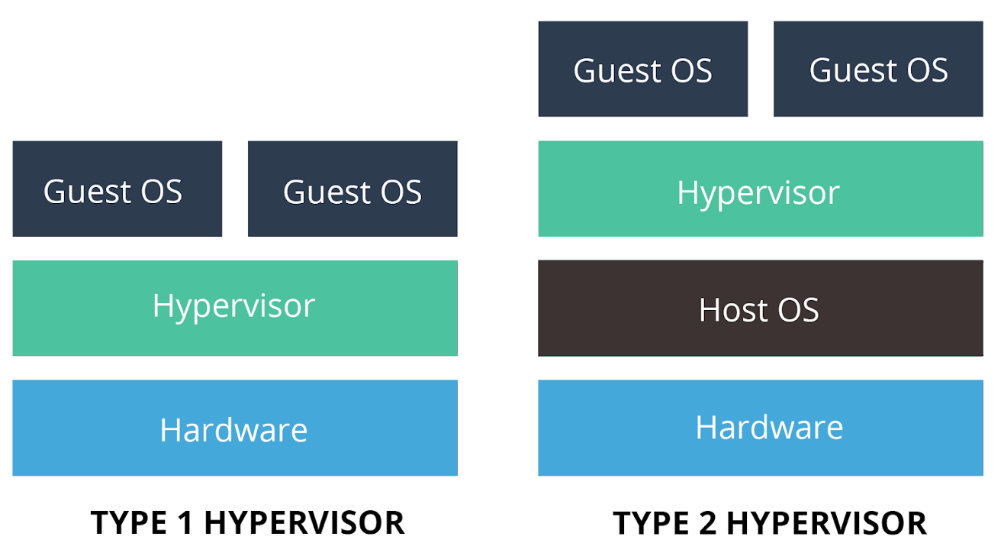
\includegraphics[width=0.6\textwidth]{../imgs/EdA/hipervisor.jpg}
\caption{Tipos de hipervisor}
\label{fig:hipervtypes}
\end{figure}

\subsubsection{KVM}
KVM (Kernel Virtual Machine)~\cite{kvm} es una tecnología de virtualización open source que convierte el kernel de Linux en un hipervisor de Tipo 1 que se puede usar para la virtualización. Las KVM tienen todos los elementos necesarios de un SO porque forman parte del kernel de Linux. Cada máquina virtual se implementa como un proceso habitual de Linux. Al ser un hipervisor de Tipo 1 ofrece un mejor rendimiento. 

\begin{figure}[h]
\centering
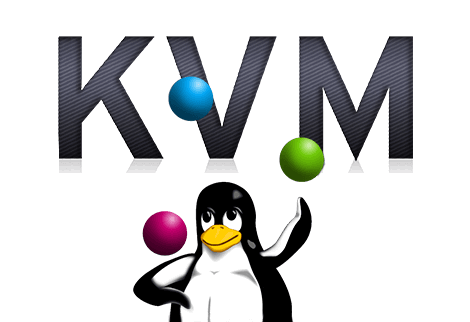
\includegraphics[width=0.3\textwidth]{../imgs/EdA/kvm.png}
\caption{Logo de KVM}
\label{fig:kvm}
\end{figure}

La configuración de la máquina virtual creada se almacena internamente en un fichero XML, el cual es posible editar manualmente a posteriori si se quiere hacer algún cambio. KVM nos permite disfrutar de las ventajas del software open source: no habrá restricciones en cuanto a integración, como sí puede haberlas si se usa un software propietario como VMware; y es independiente de proveedores. Es posible instalar una GUI\footnote{Graphical User Interface} como virt-manager, que se apoya en la biblioteca libvirt (API de virtualización estándar de Linux), para facilitar su uso.

\subsubsection{VirtualBox}
VirtualBox~\cite{vbox} es desarrollado por Oracle, aunque es gratuito y open source al igual que KVM. Es un hipervisor de Tipo 2, por lo que ofrece un rendimiento inferior comparado con un Tipo 1. VirtualBox permite crear y cargar máquinas virtuales de una forma muy sencilla, lo que hace que sea la alternativa elegida por muchos usuarios. Su asistente ofrece algunos valores sugeridos para tipos específicos de máquinas virtuales durante la creación de estas, pero su gestión final se produce en una configuración posterior.

\begin{figure}[h]
\centering
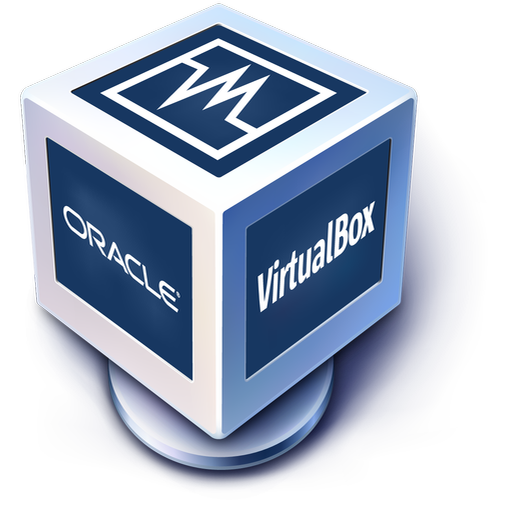
\includegraphics[width=0.2\textwidth]{../imgs/EdA/vbox.png}
\caption{Logo de VirtualBox}
\label{fig:vbox}
\end{figure}

Una ventaja de VirtualBox son las instantáneas, que permiten tomar una imagen de la máquina virtual en un momento dado. La imagen conserva la máquina virtual, lo que permite volver a ese momento específico.

VirtualBox ofrece un soporte muy completo. Tiene versiones para Windows, Linux, Macintosh y Solaris, y puede ejecutar un amplísimo número de sistemas operativos invitados, incluidos Windows, macOS, Linux, DOS, Solaris u OpenBSD.

\clearpage

\subsubsection{VMWare}
VMware~\cite{vmware} es un software comercial, lo que significa que si queremos aprovechar al máximo todas sus herramientas y configuraciones, debemos pagar por la licencia de uso. Aquí vamos a hablar de VMware Workstation Player, que es el producto gratuito de VMware para virtualización de máquinas, orientado para uso personal, doméstico y sistema educativo. 

\begin{figure}[h]
\centering

\includegraphics[width=0.2\textwidth]{../imgs/EdA/vmware.png}
\caption{Logo de VMware}
\label{fig:vmware}
\end{figure}

En comparación con VirtualBox, VMware Workstation Player es una experiencia más fluida y ágil, y ofrece mejor soporte y estabilidad para una amplia gama de hardware. Está disponible para Windows y Linux y también admite todo tipo de sistemas invitados.~\cite{versus}

Además, VMware Workstation Player sí permite personalizar toda la configuración durante el proceso de creación de la máquina virtual. La diferencia no es mucha, pero significa que la máquina virtual está lista para ejecutarse después de finalizar el asistente, en lugar de tener que realizar más configuraciones una vez que se completa.

Por el contrario, no admite instantáneas o puntos de control. Puede suspender temporalmente el sistema operativo invitado para reanudar desde un punto específico, pero no es tan completo como la creación de un historial de imágenes para la máquina virtual.

\subsection{Virtualización en contenedores}
\subsubsection{LXC}
\subsubsection{Docker}
\section{Tecnologías de aprovisionamiento}
\subsection{Aprovisionamiento estático}
\subsubsection{Docker}
\subsubsection{Vagrant}
\subsection{Aprovisionamiento dinámico}
\subsubsection{Chef}
\subsubsection{Ansible}
\section{Tecnologías de orquestación}
\subsubsection{Docker Compose}
\subsubsection{Kubernetes}
\subsubsection{Terraform}
\subsubsection{A}
